\section{Heuristics Algorithms}
\subsection{Heuristics Algorithms Design Formulation of SeVN }
\label{sub:SeVNDesignFormulation}
With the discussion above, for a given N-nodes VNR, SeVN is designed within augment graph $G^*$ of N+k nodes through properly selecting the necessary nodes or links between these nodes and dimensioning the resources requirements associated with these nodes and links.

Our design objective is to minimize the total amount of such resources(startup node number, node computing, edge bandwidth) while still guaranteeing that if a node fails (that is, the node and its adjacent links are removed in the graph $G^*$) virtual network request's topological graph still keep integration of graph $G$ topological structure and insist normal work, we can still assign each node/link of VN to a node/link of the SeVN, that has sufficient node computing and edge's bandwidth resources respectively. It is our objection that firstly minimize number of start-up backup nodes, then minimize node computing resource, last minimize edge bandwidth resource to construct function node fault tolerant graph $G^*$.

Furthermore, there are two different cases. If re-embedding or migrating the unaffected node(un-failed node) is allowed for failure recovering, it is known as the FD-SeVN design problem. Otherwise, after each failure, if the failed node is restored in the only one backup node without migrating other unaffected node, it is referred to as the FI-SeVN design problem. Generally speaking, designing FD-SeVN is a combinatorial optimization problem and needs to be investigated in depth, while FI-SeVN exists exclusively and could be figured out easily.


\subsection{Design Procedure}

%这样转可以还原的。为什么。
In this section, we propose a heuristic algorithms for FD-SeVN problem, as well as an SeVN problem's algorithm with resources sharing consideration fitting for both FD-SeVN and FI-SeVN.

Decompose topological graph of  virtual network $VN$ into N star structure $STAR$, construct match relationship between star structures. This match relationship is corresponding node transform cost relationship.

However, as a matter of fact, computing the minimum additional resources needed to convert one attributed graph to another (hereafter called graph alignment problem, GAP) is an NP-complete problem which could be reduced from the Graph Edit Distance problem \cite{justice2006binary}. Therefore, we propose a heuristic algorithms in detail, and we first decompose a graph to a set which contains star structures which retains certain structural information of the graph of embedded virtual network. Then, the graph alignment cost could be approximated by the matching cost(transform cost) between two graphs based on their star representations. This approach is elaborated as follows.


The general idea of the heuristic for FD-SeVN design is to consider the failure of primary nodes in virtual network node's label sequentially, and in each step, compute the minimum additional resources needed to reassign the task graph based on an incremental approach (i.e., recovering from the current node failure should take not only the survived primary nodes/links resources into consideration, but also the survived redundant resources reserved for previous node failure). After iteratively execute all the node failures, SeVN is constructed within the Star Structure with the added redundant resources in each step. Generally speaking, select a optimal node $v_i$ to minimum additional resource with respect to every steps.(Min value for every step )


%This translates to ensuring that every backup node has guaranteed bandwidth to all neighbors of all critical nodes.

Redistribute physical resource corresponding to augment graph $G^i$  with additional computational and bandwidth resource. concrete step is that apply for computational resource for virtual nodes and complete path around bandwidth for virtual edges.


%At the same time, for the task graph reassigning approach in
%Edit Grid, we also introduce the permutation matrices, which is
%an (N+1)×(N+1) orthogonal matrix having PPT = PT P = I
%(where I is the identity matrices), to indicate the corresponding
%state vector transformation of Edit Grid. Assume at this point
%that the initial state of the Edit Grid η0 contains the given task
%graph in its standard placement. And we have another state η1
%such that it describes task graph situated on the Edit Grid in a
%different way as shown in Fig. 3(c), as well as its state vector
%shown in Table I. Based on the knowledge in graph theory,
%the two graphs corresponding to these different states of Edit
%Grid are isomorphic [14] which suggests that there is a bijection
%between these two attributed graphs. So, we could employ
%permutation matrices to implement task graph reassignment in
%Edit Grid. For example, with the following Edit Grid state η0 :


\subsection{FD-SeVN Algorithm}
\subsubsection{Graph Decomposition}
Star Structure: A star structure s is an attributed, single-level, rooted tree which can be represented by a 7-tuple $star=(v^*,c^*,C^*,f^*,F^*,L^*,B^*)$ as shown in Figure \ref{fig:StarRepresentation}, where $v^*$ is the root node, $c^*$ is the  node's demand computing, $C^*$ is the node's remain computing capacity could be resigned again, $f^*$ is the node's function type, $F^*$ is function type set of the node, $L^*$ is other all nodes  adjacent with nodes $v^*$, $B^*$ is the bandwidth of each link $e_{ij}$ associated with the root node $v^*$. Edges exist between the root node and its adjacent nodes, and no edge exists among its adjacent nodes.

More exactly, for node $v_i$ in an attributed graph  $G^V (V^V,E^V,f^V,F^V,L^V,C^V,B^V,M^V)$, we can generate a star structure $star_i$ corresponding to $v_i$ in the following way, $star_i=(v^V_i,c^V_i,C^V_i,f^V_i,F^V_i,L^V_i,B^V_i)$ where $f^V_i$ is a function type $f_i$ running in node $v_i$, $F^V_i=\{f_{j}|$ for all $f_j$ belong node $v_i$ function set$\}$.  $L^V_i=\{v_j|$ for all nodes $v_j$  adjacent with node $v_i\}$, $B^V_i=\{b_{i,j}| $ for all $e_{i,j}\in L^V_i\}$. Accordingly, we can derive $N$ star structures from topological graph of substrate network with embedded virtual network of N nodes (we uniformly discuss all N virtual nodes fail). In this way, topological graph of embedded virtual network can be transformed to a  star structure. A quintesfntial example should be cited that construct $star_2$ corresponding to node $v_2$, $star_2=(v_2,3,7,f_2,\{f_2,f_3\},\{v_1,v_3\},\{b_{21}=4,b_{23}=6\})$, virtual node $v_1$ correspond star structure $star_1=(v_1,2,5,f_1,\{f_1\},(v_2,v_3,v_4),\{b_{12}=4,b_{13}=5,b_{14}=3\})$.
%, $C^*$ is the computation resource requirement of every nodes, $C^n=\{C^n_{u}|$for all $e_{n,u}\in E\}$
%\begin{figure}
%\centering
%% Requires \usepackage{graphicx}
%\includegraphics[width=3in]{fig/GraphDecomposition}\\
%\caption{Graph Decomposition}\label{fig:GraphDecomposition}
%\end{figure}

\subsubsection{Match Items}
Based on the topological graph of the embedded virtual network, we construct star structure set $STAR^L$, which erase some star structure corresponding to one substrate node without embedding virtual node. when calculating the virtual node $v_i$ which map to substrate node $s_i$ failure, constructing star structure set $STAR^R$ with erasing the node $v_i$ and the edge adjacent with node $v_i$ as shown in Fig.\ref{fig:StarRepresentation}.
\begin{figure}
\centering
% Requires \usepackage{graphicx}
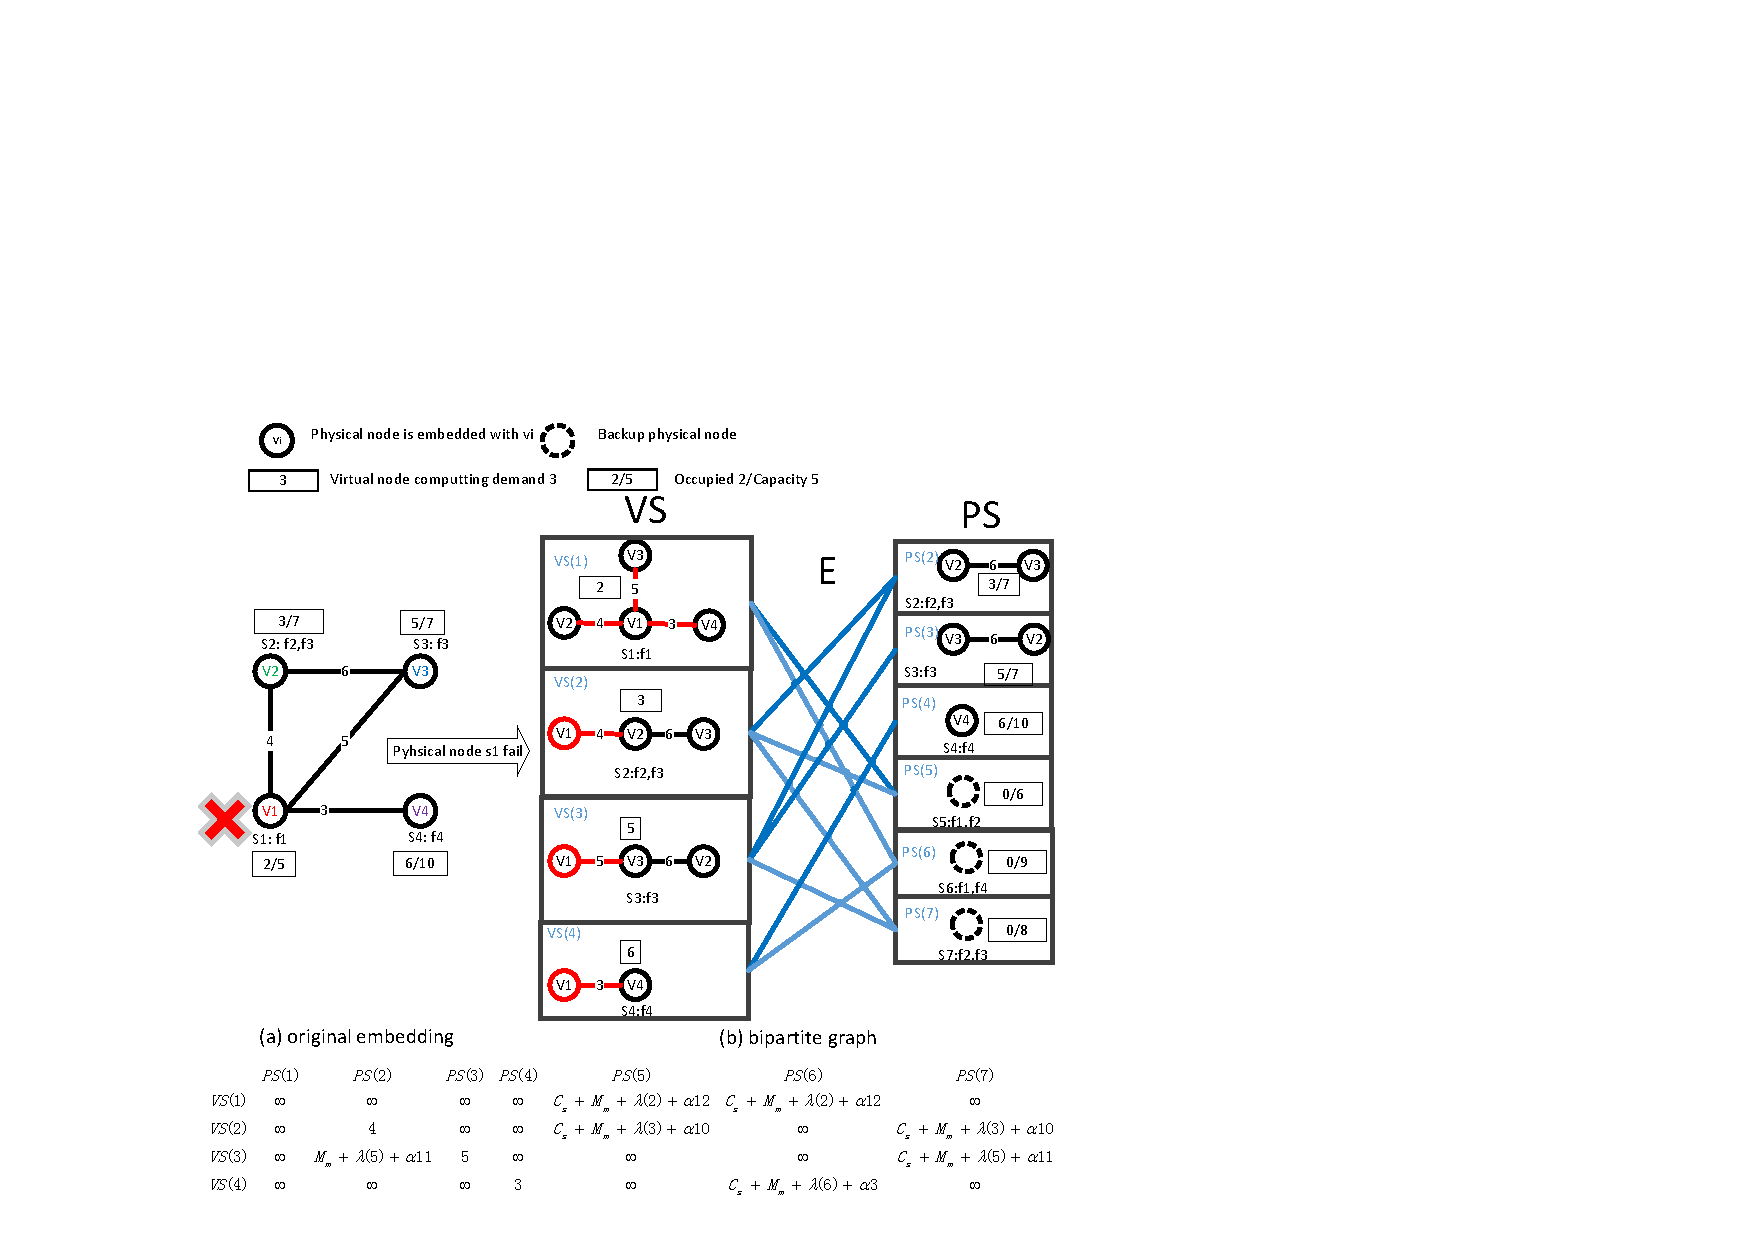
\includegraphics[width=3in]{Fig/StarRepresentation}\\
  \caption{The star representation of the embedded virtual network ($STAR^L$) and residual task graph after failure of node $v_1$ ($STAR^R$);}\label{fig:StarRepresentation}
\end{figure}
\subsubsection{Alignment Cost Matrix}
Due to the particularity of star structure, the alignment cost between two star structure set can be computed easily as below. For the two star structures $star^L_i$ and $star^R_j$ which is from $STAR^L$ and $STAR^R$ respectively, if node $f_i^V$ of $star^L_i$  is not included in $F^V_j$, the alignment cost of $star^L_i$ to $star^R_j$ is $\infty$, otherwise the alignment cost of $star^L_i$ to $star^R_j$ is
%equation \ref{equ:alignmentcost}:
%\begin{equation}\label{equ:alignmentcost}
\[\lambda(star^L_i,star^R_j)=\sum\limits_{v_u\in L_i \cap L_j}\gamma|b_{i,u}-b_{j,u}|_0+\newline
\sum\limits_{v_u\in L_i - L_j}\gamma b_{i,u}+\beta|c_i-c_j|_0+ \delta(v_i,v_j)+\theta(v_j)\]
%\end{equation}
where $\delta$, $\theta$ and $|x|_0$ is defined as follows:

$\delta ({v_i},{v_j}) = \left\{ \begin{array}{l}
{\rm{M_{m}}}\\
0
\end{array} \right.\begin{array}{*{20}{c}}
v_i\neq v_j\\
{otherwise}
\end{array}$

$\theta ({v_j}) = \left\{ \begin{array}{l}
{\rm{C_{s}}}\\
0
\end{array} \right.\begin{array}{*{20}{c}}
v_j\ is\ free\\
{otherwise}
\end{array}$

$|x|_0 = \left\{ \begin{array}{l}
{x}\\
0
\end{array} \right.\begin{array}{*{20}{c}}
if\ x\geq 0\\
{if\ x\leq 0}
\end{array}$

$\delta(v_i,v_j)\neq 0$ indicates that  root node $v_i$ should be reallocated to node $v_j$. $M_m$ is migration cost, $C_s$ is startup new node cost.we define $\lambda(star_i,star_j)$ according to graph edit distance\cite{sanfeliu1983distance}. In mathematics and computer science, graph edit distance (GED) is a measure of similarity (or dissimilarity) between two graphs.

In this way, both the topological graph of  embedded virtual network and the residual graph are composed to two star structure sets. With such a graph decomposition once a specific virtual node failure, an alignment matrix of the two star structure set could be constructed based on the alignment cost definition above. Therefore, the proposed GAP could be transformed to a (multiple knapsack problem) which will be investigated in the following part. For example, the alignment cost matrix when virtual network $v_1$ fail as follow.
\begin{equation*}
\tiny{
 {\begin{array}{*{20}{c}}
&R_{S_{2}}&R_{S_3}&R_{S_4}&R_{S_5}&R_{S_6}&R_{S_{7}}\\
{L_{V_1}}&\infty&\infty&\infty&\fbox{$C_{s}$+(2)+12}&C_{s}+(2)+12&\infty\\
L_{V_2}&\fbox{4}&\infty&\infty&C_{s}+(3)+10&\infty&C_{s}+(3)+10\\
L_{V_3}&M_{m}+(5)+11&\fbox{5}&\infty&\infty&\infty&C_{s}+(5)+11\\
L_{V_4}&\infty&\infty&\fbox{3}&\infty&C_{s}+(6)+3&\infty\\
\end{array}}
}
\label{lab:Node1FaliureAlignmentMatrix}
\end{equation*}

To elaborate this approach, Figure \ref{fig:StarRepresentation} shows how the 4-nodes VN be decomposed into a set of four star structures (shown as $STAR_L$ ), and each containing a primary task node (also called root node which is highlighted and color as blue), its adjacent links and its neighboring nodes.

\subsection{Multiple Knapsack Problem}
Based on the discussion above, the computation problem of minimal graph alignment cost is transformed to solving optimal multiple knapsack problem, which is one of the fundamental combinational optimization problems. In our case, there are two sets of vertices corresponding to the two sets of star structure of $STAR_L$ and $STAR_R$ respectively, and the weight of the edge between star structures of $STAR_L$ and $STAR_R$ is the alignment cost between the corresponding two stars.

Firstly, we proposed the formalization of the multiple knapsack problem as follow:

$M_{ij}=1(1\leq i\leq n,1 \leq j \leq m)$ represent that whether the i-th virtual node map the j-th substrate node, n and m denote virtual node's size and substrate node's size respectively.

$Cost_{ij}(1\leq i\leq n,1 \leq j \leq m)$ represent that the cost of i-th virtual node map the j-th substrate node. $\infty$ represent that there is not map relationship.

$c_i(1\leq i\leq n)$ represent that the i-th virtual node demand computational resource, $C_i(1\leq i\leq m)$ represent that the i-th substrate network maximum useful computation resource.

Objection: minimum $Cost_{ij}*M_{ij}$

constraints: $\sum\limits_{1\leq j\leq m} M_{ij}=1$,$\sum\limits_{1\leq i\leq n} c_i*M_{ij}\leq C_j$

\subsubsection{Dynamic Programming Equation}
\label{lab:DynamicProgrammingEquation}
We propose a dynamic programming equation method for solving the multiple knapsack problem. Assume $C_1,C_2,\ldots,C_n$, $C$ are strictly positive integers. Define $dp[i][{C_1}][{C_2}] \ldots [{C_m}]=0$ to be the minimum value that can be attained with n capacity variables  which less than or equal to $C_i$ using items up to knapsack i.

Initial state $dp[i][{C_1}][{C_2}] \ldots [{C_m}]=0$ is firstly assigned as infinity $\infty$. $dp[i][{C_1}][{C_2}] \ldots [{C_m}]=0$ when there is no any virtual node which is confirmed to map into another node. The total cost of current state is zero. $dp[i][{C_1}][{C_2}] \ldots [{C_m}]$ when  i nodes is succeeded to be mapped another nodes. The total cost of current state is minimal cost from optimal node location.

We can define $dp[i][{C_1}][{C_2}] \ldots [{C_m}]$ recursively as in Equation \ref{equ:statetransferequation}, when put i-th node into another node, in this situation, the current state is calculated from former i-1 nodes are succeeded to be mapped.

\begin{equation}
\label{equ:statetransferequation}
\min \left\{ \begin{array}{l}
dp[i - 1][{C_1-c_i}][{C_2}] \ldots [{C_m}]+\lambda(star^L_i,star^R_1)\\
dp[i - 1][{C_1}][{C_2-c_i}] \ldots [{C_m}]+\lambda(star^L_i,star^R_2)\\
...\\
dp[i - 1][{C_1}][{C_2}] \ldots [{C_m-c_i}]+\lambda(star^L_i,star^R_n)
\end{array} \right.
\end{equation}

dynamic programming method  could be applied to solve the multiple knapsack problem whose time complexity is $O[(n+b)*n*\prod_{i=1}^{n+b}C^i]$, which is pseudo-polynomial time. Space complexity is $O[n*\prod_{i=1}^{n+b}C^i]$.








